
\begin{frame}{Computational reproducibility should be easy...}

  % 
  \begin{columns}
    %
    \begin{column}{.5\textwidth}
      \begin{figure}
        \centering
        \includegraphics[width=0.85\textwidth]{%
          monkey.png}  %
      \end{figure}
      
    \end{column}
    %
    \begin{column}{.5\textwidth}

      \begin{figure}
        \centering
        \includegraphics[width=0.85\textwidth]{%
          computer.png}  %
      \end{figure}
      
    \end{column}
  \end{columns}

  \begin{columns}
    %
    \begin{column}{.5\textwidth}
      \begin{center}
        Hard
      \end{center}
      
    \end{column}
    %
    \begin{column}{.5\textwidth}
      \begin{center}
        Easy?
      \end{center}
      
    \end{column}
  \end{columns}
  
\end{frame}


\begin{frame}{Computational reproducibility should be easy...}

  \vspace{0.7cm}
  
  \begin{itemize}[leftmargin=1.2cm, rightmargin=1cm]

    \itemsep10pt

  \item[1.] cheap and universal access to computers (as opposed to a lab)
  \item[2.] running code is inexpensive and unproblematic (compared to replicating an experiment)
  \item[3.] can easily share code \& data that allow direction reproduction
    % 1. everyone has a computer (as opposed to a lab setup) and
    %    running code is inexpensive and unproblematic compared
    %    to replicating experiment
    % 2. can share all the code (~5MB) opposed to sharing a full
    %    lab (impossible)
    
    
  \end{itemize}


  

  % 
  \begin{columns}
    %
    \begin{column}{.625\textwidth}
      \minipage[c][0.45\textheight][s]{\columnwidth}

      \vspace{1.2cm}
      \begin{center}
        \textit{Is a there a reproducibility crisis\\ in computational research?}
      \end{center}        
      
      \endminipage      
    \end{column}
    %
    \begin{column}{.375\textwidth}
      \onslide<1->
      \vspace{-1cm}
      \begin{figure}
        \centering
        
\includegraphics[width=\textwidth]{%
          img/computer.png} %
      \end{figure}
      
      
      
    \end{column}
  \end{columns}
  


  \pnote{
    
    But as many of you have probably experienced,\\
    code is often not shared.\\

    But surely, journals implementing policies \\
    should help?

    Well, let's take a look:
    
  }


  
  
\end{frame}



\begin{frame}{Sharing of code \& data mandatory in many journals}

  
  \begin{figure}
    \centering
    \includegraphics<1>[width=0.95\textwidth]{%
      img/science_policy.png} %
    \includegraphics<2>[width=0.95\textwidth]{%
      img/science_policy_t1.png} %
    \includegraphics<3>[width=0.95\textwidth]{%
      img/science_policy_t2.png} %
  \end{figure}

  \vspace{0.4cm}
  
  \begin{flushright}
    \small Policy of \textit{Science} since February 11, 2011
  \end{flushright}

  \pnote{
    
    Now that we established computational reproducibility\\
    should be simple and journals are demanding\\
    sharing anyway, we're good, right?

    How effect is such an policy?
    
  }
  
\end{frame}

\begin{frame}{}
  
  \begin{figure}
    \centering
    
\includegraphics[width=0.875\textwidth]{%
      img/stodden2018_cover3.png} %
  \end{figure}
  
  \vspace{0.015cm}

  \begin{center}
    Out of 206 computational studies in \textit{Science} since 2011, \\
    26 provided code \& data directly  
  \end{center}
  

  \source{\cite{Stodden2018}}

  \pnote{
    
    To the remaining 180 studies \\
    the authors sent Emails asking \\
    for the code for the studies
    
  }

  
\end{frame}


\begin{frame}{A few responses...}
  
  \begin{figure}
    \centering
    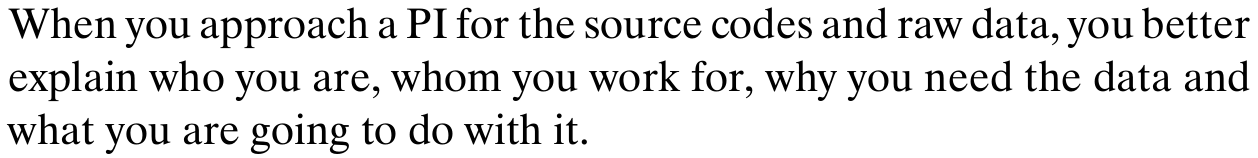
\includegraphics[width=0.95\textwidth]{%
      img/stodden2018_re1.png} %
  \end{figure}

  \begin{figure}
    \centering
    
\includegraphics[width=0.95\textwidth]{%
      img/stodden2018_re2.png} %
  \end{figure}

  \begin{figure}
    \centering
    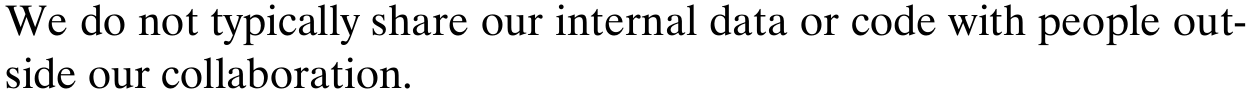
\includegraphics[width=0.95\textwidth]{%
      img/stodden2018_re3.png} %
  \end{figure}

  \source{\cite{Stodden2018}}
  
\end{frame}



\begin{frame}{\large   Of $N=206$ articles published in \textit{Science} since 2011...}


  \begin{figure}
    \centering
    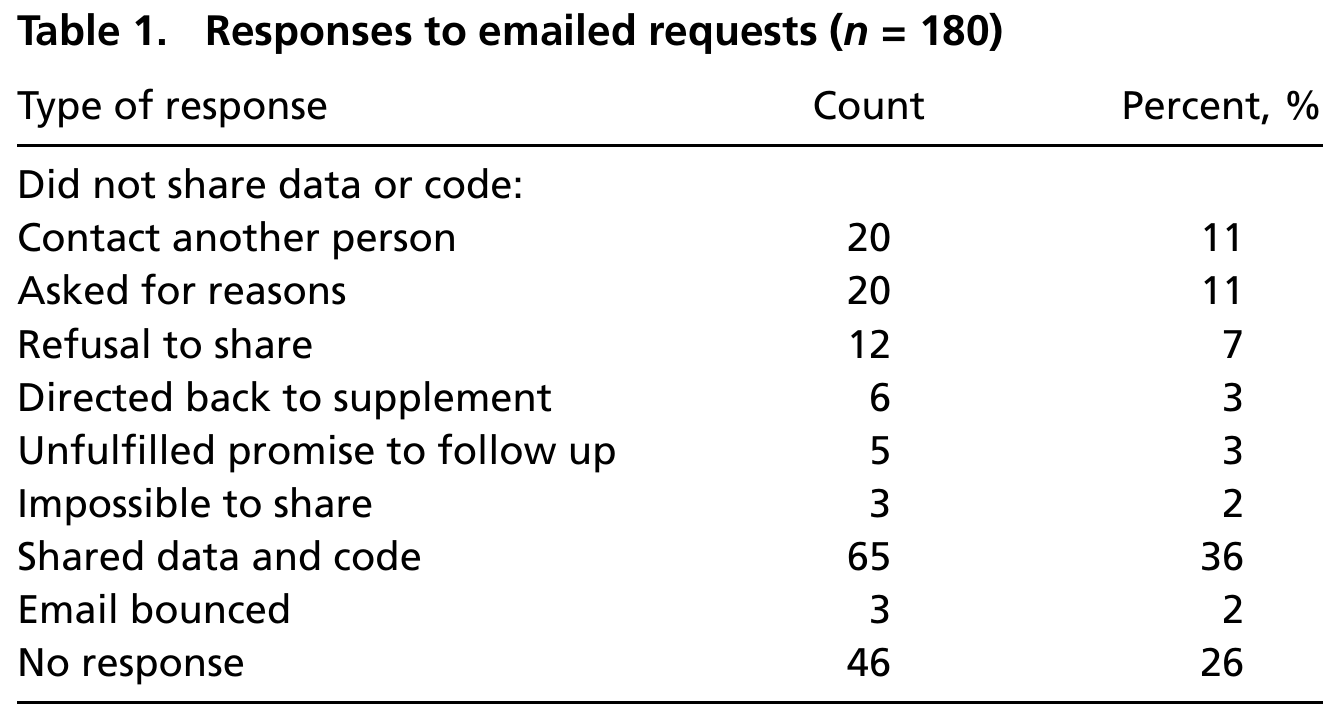
\includegraphics[width=0.9\textwidth]{%
      img/stodden2018_table1.png} %
  \end{figure}

  \vspace{0.1cm}
  
  \begin{center}
    $\Rightarrow$ Code \& data could be retrieved for 91 out of 206 studies.    
  \end{center}

  \source{\cite{Stodden2018}}
  
\end{frame}


\begin{frame}{}%Open Source for Neuroscience}

  \begin{figure}
    
\includegraphics[width=0.95\textwidth]{%
      img/open_source_neuroscience.png} %
  \end{figure}
  
\end{frame}



\begin{frame}{Open Source for Neuroscience}

  \begin{figure}
    \centering
    %% \includegraphics<1>[width=0.9\textwidth]{%
    %%   img/open_source_neuroscience.png} %
    \includegraphics<1>[width=\textwidth]{%
      img/pledge_2.png} %
    \includegraphics<2>[width=\textwidth]{%
      img/pledge_2_t1.png} %
  \end{figure}

  \onslide<1->
  \begin{center}
    \href{http://opensourceforneuroscience.org/}{opensourceforneuroscience.org/}
  \end{center}

  \pnote{
    
    As of 2018/04: 200 neuroscientist have made this pledge
    
  }
  
\end{frame}



\begin{frame}{A slide of hope}

  Researchers are committing to sharing the code and data. Journals have to demand

  This is .

  With this reproducibility in computational research is no longer an issue, right?
  
  
\end{frame}




\begin{frame}{Reproducibility when code was available}

  \vspace{0.05cm}
  
  56 out of 91 studies were judged as \textit{potentially reproducible}

  \vfill
  
  \onslide<2->
  \begin{tabular}{|p{0.9\textwidth}}
    However, even when code was available, more than half of studies were reproducible only with \textit{\textcolor{red}{significant effort!}}  
  \end{tabular}	     

  \vfill


  \onslide<3-6>{

    Problems:
  \vspace{-0.15cm}

  \begin{columns}[T]
    %
    \begin{column}{.5\textwidth}
      %% \minipage[c][0.3\textheight][s]{\columnwidth}
      \begin{itemize}[leftmargin=0.75cm]

      \item<3->[-] impossible to reproduce (missing code, data or methodology)
      \item<4->[-] required tedious effort (e.g.\ download large number of individual data sets)
        
        
      \end{itemize}
      %% \endminipage      

    \end{column}
    %
    \begin{column}{.5\textwidth}
      %% \minipage[c][0.3\textheight][s]{\columnwidth}
      
      \begin{itemize}[leftmargin=*]
      \item<5->[-] required intellectual effort (e.g.\ knowledge of past articles, implementing given pseudo code)
      \item<6->[-] required tweaking (e.g.\ mising parameters, minor methods steps)
            
      \end{itemize}
      %% \endminipage
      
    \end{column}
    %
  \end{columns}
  \vspace{0.2cm}}

  \source{\cite{Stodden2018}}
    
\end{frame}



\begin{frame}{Reproducibility when code was available}

    \begin{figure}
      \centering
      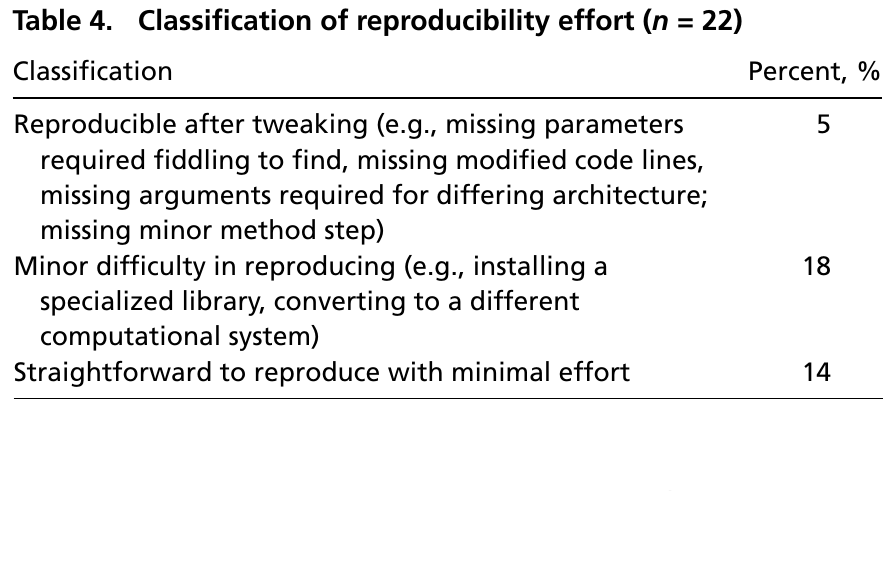
\includegraphics[width=0.85\textwidth]{%
      img/stodden2018_table4_3-3.png} %
    \end{figure}

    \vspace{-1.25cm}
  
\begin{center}
      Computational reproducibility remains difficult even \\when code is available!
      
\end{center}
  
    
\end{frame}






\begin{frame}{\large Measuring Reproducibility in Computer Systems Research}

  \begin{figure}
    \centering
    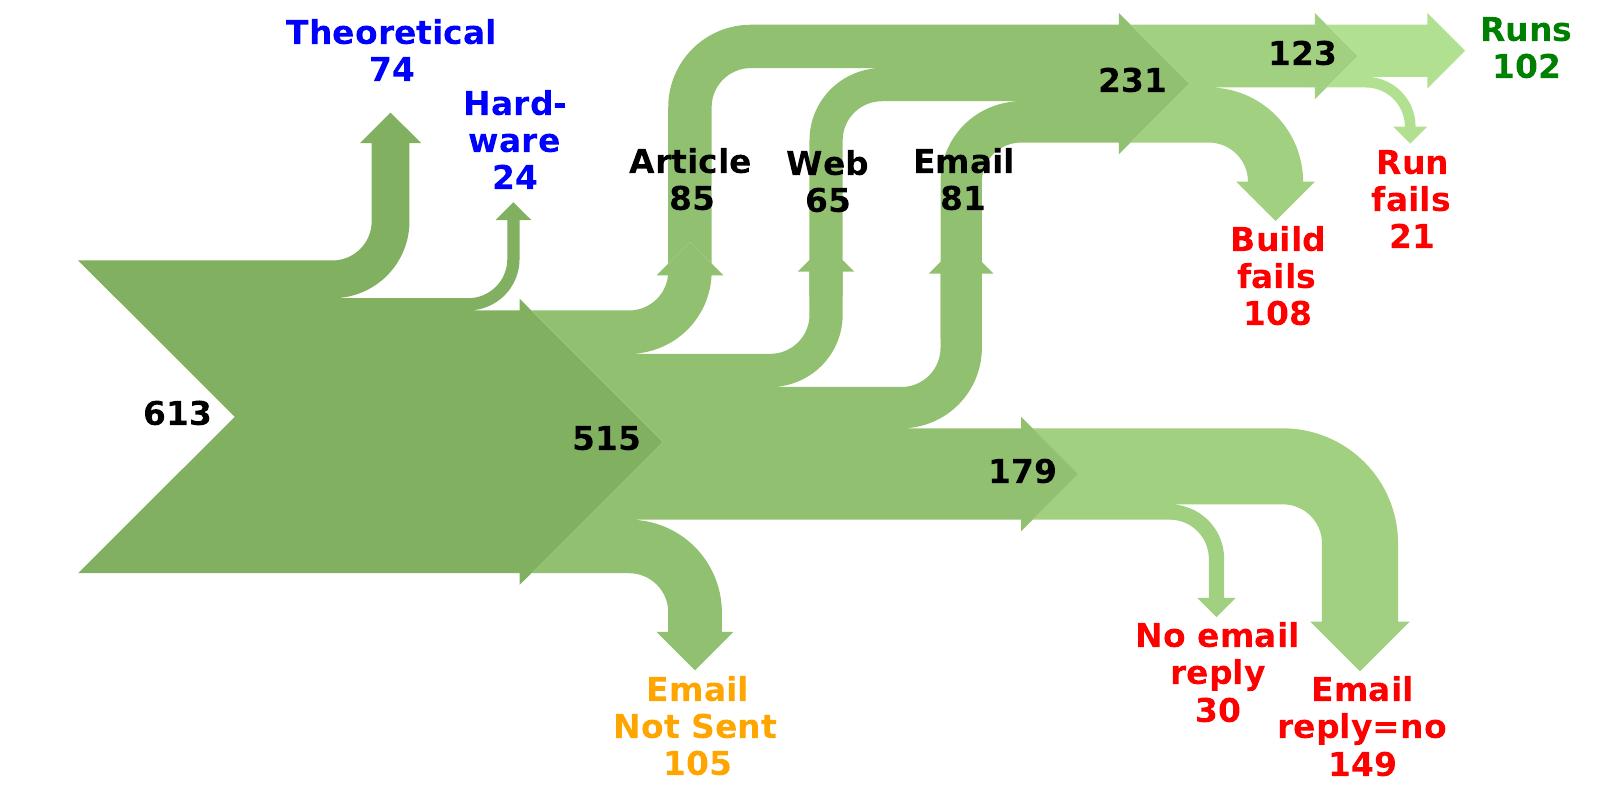
\includegraphics[width=\textwidth]{%
      img/collberg2013_results3.png} %
  \end{figure}
  

  \source{\cite{Collberg2013}}

  \pnote{
    
    613 papers from \\
    - 8 conferences \\
    - 5 journals

    30 minutes of programmer time to try \\
    make build compile/run
    
    Orange: Don't send more than one email to any author \\
    (if author had multiple publications)

    Even if build runs does not even try verify results! \\
    How many more papers will fall off?
    
  }
  
  
\end{frame}


\begin{frame}{\large Why wasn't code available? (Or, the dog ate my program)}
  
  
  
\end{frame}
